\documentclass[11pt]{examdesign}
\usepackage[spanish]{babel}
\OneKey
\usepackage[utf8]{inputenc}
\usepackage[T1]{fontenc}
\usepackage{amsmath}
\usepackage{pifont}
%-----------------------------------------------------------------------------------------------
%\usepackage{gfsartemisia-euler}
\usepackage{graphicx}
\usepackage{float}
\usepackage{amscd}
\usepackage{amsfonts}
\usepackage{amssymb}
\usepackage{mathtools}
\usepackage{amsthm}
\usepackage[all]{xy}
\usepackage{enumitem}
\usepackage{multicol}
\usepackage{verbatim}
\usepackage[colorlinks=true,
linkcolor=blue,
urlcolor=red,
bookmarksopen=true]{hyperref}
\usepackage[pdftex,dvipsnames]{xcolor}
\definecolor{aqua}{rgb}{0.0, 1.0, 1.0}
\definecolor{caribbeangreen}{rgb}{0.0, 0.8, 0.6}
\definecolor{tealgreen}{rgb}{0.0, 0.51, 0.5}
\definecolor{upforestgreen}{rgb}{0.0, 0.27, 0.13}
\definecolor{napiergreen}{rgb}{0.16, 0.5, 0.0}
\definecolor{capri}{rgb}{0.0, 0.75, 1.0}
\definecolor{calpolypomonagreen}{rgb}{0.12, 0.3, 0.17}
\definecolor{azure(colorwheel)}{rgb}{0.0, 0.5, 1.0}
\definecolor{dukeblue}{rgb}{0.0, 0.0, 0.61}
\definecolor{bole}{rgb}{0.47, 0.27, 0.23}
\definecolor{gris}{gray}{0.975}
%----------------------------------------------------------------------------------------------
% Si desea utilizar \@@line para definir su propio encabezado de examen o palabras del encabezado, 
% asegúrese de usar \makeatletter y \makeatother en los lugares apropiados, de lo contrario 
% podría obtener errores.
%-----------------------------------------------------------------------------------------------
\makeatletter
% manual page 10
\begin{examtop}
	\@@line{\parbox{3in}{\classdata \\[0.5cm]
			\textcolor{upforestgreen}{\textbf{\underline{T.P.N$^\circ$}}~\fbox{\textsc{5}}}: \examtype}
		%                  ^^^^^^
		\hfill
		\parbox{3in}{\normalsize \namedata}}
	\bigskip
\end{examtop}
% manual page 10
\def\namedata{\textcolor{upforestgreen}{\underline{\textbf{Estudiante}}}:\hrulefill \\[\namedata@vspace]
	\textcolor{upforestgreen}{\underline{\textbf{Curso y División}}}: 1$^\circ$ Año \\[\namedata@vspace]
	\textcolor{upforestgreen}{\underline{\textbf{División}}}: I
	\\[\namedata@vspace]
	\textcolor{upforestgreen}{\underline{\textbf{Profesor}}}: Ferreira, Juan David \\[\namedata@vspace]
	\textcolor{upforestgreen}{\underline{\textbf{Fecha}}}: 22-06-2020 al 29-06-2020
}
% manual page 11        
\begin{keytop}%
	\@@line{\hfill \Huge\texttt{\textcolor{upforestgreen}{Respuestas 
				Trabajo Práctico N$^\circ$~\fbox{\textsc{5}}}} \hfill}
	\bigskip
\end{keytop}%
\makeatother


\examname{\textcolor{upforestgreen}{\underline{\textbf{Actividedes de Integración}}}}
%\SectionPrefix{Sección \arabic{sectionindex}. \space}
%\SectionPrefix{Sección \Alph{sectionindex}. \space}
%\SectionPrefix{Punto \Alph{sectionindex}. \space}
%\SectionPrefix{Punto \arabic{sectionindex}. \space}
%\SectionPrefix{Ejercicio \Alph{sectionindex}. \space}
%\SectionPrefix{\textcolor{upforestgreen}{\textbf{Ejercicio \arabic{sectionindex}}.} \space}
%\SectionPrefix{\textcolor{upforestgreen}{\textbf{Parte \Alph{sectionindex}}.} \space}
\SectionPrefix{\textcolor{upforestgreen}{\textbf{Parte \arabic{sectionindex}}.} \space}
%%%%%%%%%%%%%%%%%%%%%%%%%%%%%%%%%%%%%%%%%%%%%%%%%%%%%%%%%%%%%%%%%%%%%%%%%%%%%%%%%%%%%%%%%%%%%%%%%

% Este macro toma un argumento, quiere decir que dentro de las llaves vamos a colocar un estilo de
% letra para nuestro titulo. hay que saber acerca de fuentes y estilos de letras.

%%%%%%%%%%%%%%%%%%%%%%%%%%%%%%%%%%%%%%%%%%%%%%%%%%%%%%%%%%%%%%%%%%%%%%%%%%%%%%%%%%%%%%%%%%%%%%%%%

%\SectionFont{\Large\rmfamily}
%\SectionFont{\Large\sffamily}
%\SectionFont{\Large\ttfamily}
%\SectionFont{\Large\mdseries}
%\SectionFont{\Large\bfseries}
%\SectionFont{\Large\upshape}
%\SectionFont{\Large\slshape}
%\SectionFont{\Large\itshape}
%\SectionFont{\Large\scshape}

%%%%%%%%%%%%%%%%%%%%%%%%      Nos da los margenes                        %%%%%%%%%%%%%%%%%%%%%%%%%%%
%%%%%%%%%%%%%%%%%%%%%%%%%     Funciona igual que el paquete geometry     %%%%%%%%%%%%%%%%%%%%%%%%%%%
\Fullpages

\ContinuousNumbering
%%%%%%%%%%%%%%%%%%%%%%%%%%%%%%%%%      RESPUESTAS CORTAS     %%%%%%%%%%%%%%%%%%%%%%%%%%%%%%%%%%%%%%%%
%\ShortKey

\DefineAnswerWrapper{}{}
%%%%%%%%%%%%%%%%%%     NUMERO DE VERSIONES DEL EXAMEN FILA A, FILA B, FILA C, ETC     %%%%%%%%%%%%%%%
\NumberOfVersions{1}
%%%%%%%%%%%%%%%%%%%%%%%%%%%%%%%%%%%%%%%%%%%%%%%%%%%%%%%%%%%%%%%%%%%%%%%%%%%%%%%%%%%%%%%%%%%%%%%%%
% Este macro toma un argumento, quiere decir que dentro de las llaves vamos a colocar un estilo de letra para nuestro titulo. hay que saber acerca de fuentes y estilos de letras.
%%%%%%%%%%%%%%%%%%%%%%%%%%%%%%%%%%%%%%%%%%%%%%%%%%%%%%%%%%%%%%%%%%%%%%%%%%%%%%%%%%%%%%%%%%%%%%%%%

\class{{\textcolor{upforestgreen}{\Large\textbf{E.P.E.S. Nro 51 ``J. G. A.''}}\\[0.5cm]
		\textcolor{upforestgreen}{{\Large \textbf{Matemática}}}}}

\begin{document}
    %-------------------------------             SHORT ANSWER        ------------------------%
    \begin{shortanswer}[title={Completar los siguientes cuadros siguiendo el ejemplo dado:},
    	rearrange=no,resetcounter=no]
    	
        
        \begin{question}
        Cada cuadro se completa la fraccion, su nombre, su expresión decimal y el porcentaje que representa, como en el ejemplo del primer renglón.
        	\begin{multicols}{2}
        		
        		% 30% de la página
        		\begin{tabular}{|c|c|c|c|}
        			\hline
        			{\scriptsize Fracción}      &{\scriptsize Expresión}&{\scriptsize Nombre}	 &{\scriptsize Expresión}
        			\\
        			&{\scriptsize Decimal}     &            &{\scriptsize Porcentual}
        			\\\hline
        			$3/4$ & $0.75$  & Tres cuartos&$75\%$
        			\\\hline
        			$1/4$ &         &           &             
        			\\\hline
        			& $0.5$   &           &
        			\\\hline
        			&         & Un quinto&
        			\\\hline
        			$1$           & $0.8$   &           &
        			\\\hline
        			$3/5$ &         &           &
        			\\\hline
        			&         &{\scriptsize siete medios}&
        			\\\hline
        		\end{tabular}
        		%\columnbreak
        		\begin{tabular}{|c|c|c|c|}
        			\hline
        			{\scriptsize Fracción}      &{\scriptsize Fracción}     &{\scriptsize Fracción}	 &{\scriptsize Fracción}
        			\\
        			&{\scriptsize Simplificada} &{\scriptsize Amplificada} &{\scriptsize Ireducible}
        			\\\hline
        			$12/20$  & $6/10$  &$30/50$  & $3/5$
        			\\\hline
        			$9/18$   &         &         &             
        			\\\hline
        			$15/45$  &         &         &
        			\\\hline
        			$28/36$  &         &         &
        			\\\hline
        			$8/9$    &         &         &
        			\\\hline
        			$1/3$    &         &         &
        			\\\hline
        			$4/20$   &         &         &
        			\\\hline
        		\end{tabular}
        	\end{multicols}
        	\begin{answer}
        		\textbf{Repuesta}: este ejercicio así planteado no tiene solución.
        	\end{answer}
        \end{question}        
    \end{shortanswer}
    
    %------------------------     COMPLETAR ESPACIOS EN BLANCOS      -----------------------%
    \begin{fillin}[title={Calcula de la manera que prefieras los siguientes porcentajes:},resetcounter=yes]
    	
    	\begin{question}
    		$40\%$ de $300 km=$\blank{woodchuck}
    	\end{question}
    	
    	\begin{question}
    		$20\%$ de $60 kg$ de panes = \blank{woodchuck}.
    	\end{question}
    	
    	\begin{question}
    		$60\%$ de $600$ empleados = \blank{woodchuck}.
    	\end{question}
    	
    	\begin{question}
    		$75\%$ de $300$ peatones =\blank{woodchuck}.
    	\end{question}
    	
    	\begin{question}
    	$12\%$ de $180$ estudiantes = \blank{woodchuck}
    	\end{question}
    	
    	\begin{question}
    		$30\%$ de $990$ pesos = \blank{woodchuck}
    	\end{question}	
    \end{fillin}
 
    %-------------------------         VERDADERO O FALSO         --------------------------------%
    \begin{truefalse}[title={\textcolor{upforestgreen}{\textbf{Parte $3$.}}	Observa las imágenes, calcula si es necesario y coloca Verdadero ó Falso según corresponda},
    	resetcounter=no,suppressprefix]
        \begin{center}
        	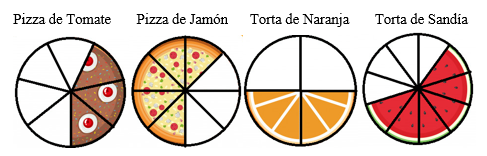
\includegraphics[width=10cm, height=4cm]{pizzas.png}
        \end{center}
    	\begin{question}
    		\answer{True} Sobra el $50\%$ de la Pizza de Tomate.
    	\end{question}
    	
    	\begin{question}
    		\answer{True}  Sobró el $60\%$ de la Torta de Sandía.
    	\end{question}
    	
    	\begin{question}
    		\answer{False} Se comieron 3$/7$ de la Pizza de Tomate.
    	\end{question}
        
        \begin{question}
        	\answer{False} Falta $6/12$ de la Torta de Naranja.
        \end{question}
        \begin{question}
        	\answer{False} Si alguien come 3 porciones de la Pizza de Jamón quedará el $25\%$.
        \end{question}
    	
    \end{truefalse}
    
    %-------------------------         short answer        --------------------------------%
    
    \begin{multicols}{2}
    	\begin{shortanswer}[title={Pensamos y reflexionamos (escribe en la carpeta tus conclusiones)},
    		,
    		rearrange=no,resetcounter=yes]
    		$\bullet$ Suponiendo que la torta de sandía estaba completa y comimos una porción de la torta en el almuerzo y otra en la cena: 
    		
    		\begin{question}
    			¿Cuántas porciones nos habremos comido?
    			\begin{answer}
    				\textbf{Respuesta}:.
    			\end{answer}
    		\end{question}
    		
    		\begin{question}
    			Si reiteramos esta situación durante 3 días seguidos: ¿Quedarán porciones? ¿Cuántas porciones quedarán?
    			\begin{answer}
    				\textbf{Respuesta}:.
    			\end{answer}
    		\end{question}
    	\end{shortanswer}
        \columnbreak
        \begin{shortanswer}[title={Pensamos y reflexionamos (escribe en la carpeta tus conclusiones)},
        	,
        	rearrange=no,resetcounter=yes]
        	
        	$\bullet$ Suponiendo que hay opciones de comer la torta de sandía y la de naranja en un cumpleaños y como una porción de cada una: 
        	
        	\begin{question}
        		¿Cuántas porciones de la torta de sandía serían?.
        		\begin{answer}
        			\textbf{Respuesta}:.
        		\end{answer}
        	\end{question}
        	
        	\begin{question}
        		¿Cuántas porciones de la torta de naranja serían?.
        		\begin{answer}
        			\textbf{Respuesta}:.
        		\end{answer}
        	\end{question}
        	
        \end{shortanswer}
    \end{multicols}
     
    %-----------------------------------------------------------------------------------------------%
    
\end{document}